\chapter{OCaml Implementation}
\thispagestyle{nohead}
\label{Implementation}

This chapter will give some details of the choices we made when implementing the \where~tool.
We decided to make \where~available as a stand-alone tool on the command-line as well as through the \why~system by imitating an orthodox SMT solver.   

The implementation of \where~makes use of various techniques and heuristics encountered when researching related premise selection and portfolio solving tools such as those described in sections \ref{sub:lrsvml} and \ref{sub:lrsvmmml} of the Literature Review.   
For example, \where's interaction with \why~is inspired by Sledgehammer's MaSh \cite{Sledgehammer} tool. MaSh uses machine learning to suggest premises based on a large corpus of learned theorems, allowing POs to be proved automatically by ATP and SMT tools. 
We aspired to Sledgehammer's ``zero click, zero maintenance, zero overhead'' philosophy in this regard: \where~should not interfere with a \why~user's normal work-flow nor should it penalise those who do not use it.

One heuristic we implemented was to call the highest ranking solver installed on the user's system from the following static ranking:
$ \text{Alt-Ergo-1.01}\linebreak > \text{CVC4} > \text{CVC3} > \text{Z3-4.4.1} > \text{Alt-Ergo-0.95.1} > \text{Z3-4.3.2} > \text{Yices} > \text{veriT} $.
We derived this ranking from the total number of POs each solver could prove (as listed in Table \ref{table:avgtimes}).
The use of a high-performing solver called initially with a short time limit value discharges easy POs.
It does this without incurring the cost of feature extraction and solver rank prediction.
This heuristic is implemented successfully in the SATzilla  \cite{SATzilla2012} portfolio solver for SAT instances where it is termed ``pre-solving''.
SATzilla has inspired the use of pre-solving in portfolio solvers for constraint / optimisation problems such as sunny-cp \cite{sunny-cp}.
This heuristic improves \where's performance and reduces its reliance on the underlying random forest prediction model. 
The process described in Algorithm \ref{algo:rank} for obtaining results from solver rankings needs to be modified to describe \where's operation:
the following algorithm (Alg. \ref{algo:where4}) only performs feature extraction if the initial solver does not solve the input program within one second. 

\begin{algorithm}
	\caption{Returning an answer and runtime from a \why~input program}
	\KwIn{$P$, a \why~program; \\ 
		$R$, a static ranking of solvers for pre-proving; \\
		$\phi$, a timeout value}
	\KwOut{$\langle A,T\rangle$ where\\$A$ = the best answer from the solvers;\\
	$T$ = the cumulative time taken to return $A$}
	\Begin{
		\tcc{Highest ranking solver installed locally}
		$S \leftarrow BestInstalled(R) $ \\			
		\tcc{Call solver $S$ on \why~program $P$ with a timeout of 1 second}	
		$\langle A,T \rangle \leftarrow Call(P, S, 1)$ \\
		\If{$A \in \lbrace Valid, Invalid \rbrace $}
			{\Return{$\langle A,T \rangle$}}
		\tcc{extract feature vector $F$ from program $P$} 
		$F \leftarrow ExtractFeatures(P) $ \\
		\tcc{$R$ is now based on program features}
		$R \leftarrow PredictRanking(F) $ \\		
		\While{$A \notin \lbrace Valid, Invalid \rbrace \wedge R \neq \emptyset$}
		{
			$S \leftarrow BestInstalled(R) $ \\	
			\tcc{Call solver $S$ on \why~program $P$ with a timeout of $\phi$ seconds}	
			$\langle A_S,T_S \rangle \leftarrow Call(P, S, \phi)$ \\
			\tcc{add time $T_S$ to the cumulative runtime}
			$T \leftarrow T + T_S$  \\
			\If{$A_S > A$}
			{
				\tcc{answer $A_S$ is better than the current best answer}		
				$A \leftarrow A_S$ }
			\tcc{remove $S$ from the set of solvers $R$}
			$R \leftarrow R \setminus \lbrace S \rbrace$}
		\Return{$\langle A,T\rangle$}} 
	\label{algo:where4}
	
\end{algorithm}

\section{Finding the minimal number of trees}
\label{sec:min-trees}

As previously discussed, the Random Forest algorithm operates by finding a prediction from each of its constituent decision trees and averaging their results.
The generalisation of these results is improved by limiting the depth of these trees.
The heuristic we used to ensure that no prediction was associated with less than five training instances was introduced in the previous chapter.

The Sci-Kit Learn implementation of the Random Forest algorithm uses 100 trees. 
When implementing our own version of the algorithm, the efficiency of deriving these predictions has to be taken into account.
For that reason, we want to minimise the number of trees which have to be traversed.

As Table \ref{table:findtrees} shows, the prediction accuracy of the model does not deteriorate significantly as the number of trees decreases. 
We decided to use 50 trees for the final OCaml implementation: it can be seen that this number represents the point where the number of trees and the model's performance reaches stability.
No significant increases in terms of Mean Average Error or Regression Error correspond to the use of more trees beyond this point.     

\begin{table}
\caption{Finding the minimal number of trees }

	\begin{tabular}{lrrrrr}
		\toprule
		\textbf{N Trees} &  \textbf{Time} & $R^2$ &  \textbf{nDCG} &    \textbf{MAE} &  \textbf{Reg-error} \\
		\midrule
		10 &     15.09 & 0.24 & 0.48 &    2.12 &       41.10 \\
		20 &     14.99 & 0.27 & 0.48 &    2.12 &       40.39 \\
		30 &     15.03 & 0.28 & 0.47 &    2.12 &       40.61 \\
		40 &     15.02 & 0.28 & 0.48 &    2.12 &       40.42 \\
		50 &     15.00 & 0.28 & 0.48 &    2.10 &       39.55 \\
		60 &     15.00 & 0.28 & 0.48 &    2.10 &       39.68 \\
		70 &     15.05 & 0.28 & 0.48 &    2.10 &       39.39 \\
		80 &     15.00 & 0.28 & 0.48 &    2.10 &       39.37 \\
		90 &     15.00 & 0.28 & 0.48 &    2.10 &       39.35 \\
		100&	 14.99 & 0.28 & 0.48 &    2.09 &       39.63 \\
		\bottomrule
	\end{tabular}
	\label{table:findtrees}

\end{table}    


\section{Encoding the random forest}
\label{sec:encoding}

We train the Random Forest model described in Sec. \ref{sec:chosen} (and refined in the previous section) on the entire training set.
The Sci-kit Learn library allows the constituent decision trees to be extracted and inspected.
We print the forest as a JSON array of trees using the data model shown in Fig. \ref{fig:json}. 
%Each \texttt{Forest} consists of an array of \texttt{Trees}, which in turn consist of an array of \texttt{Nodes}. Each node has a unique identifier which is used for navigating the tree. A \texttt{

\begin{figure}
\centering
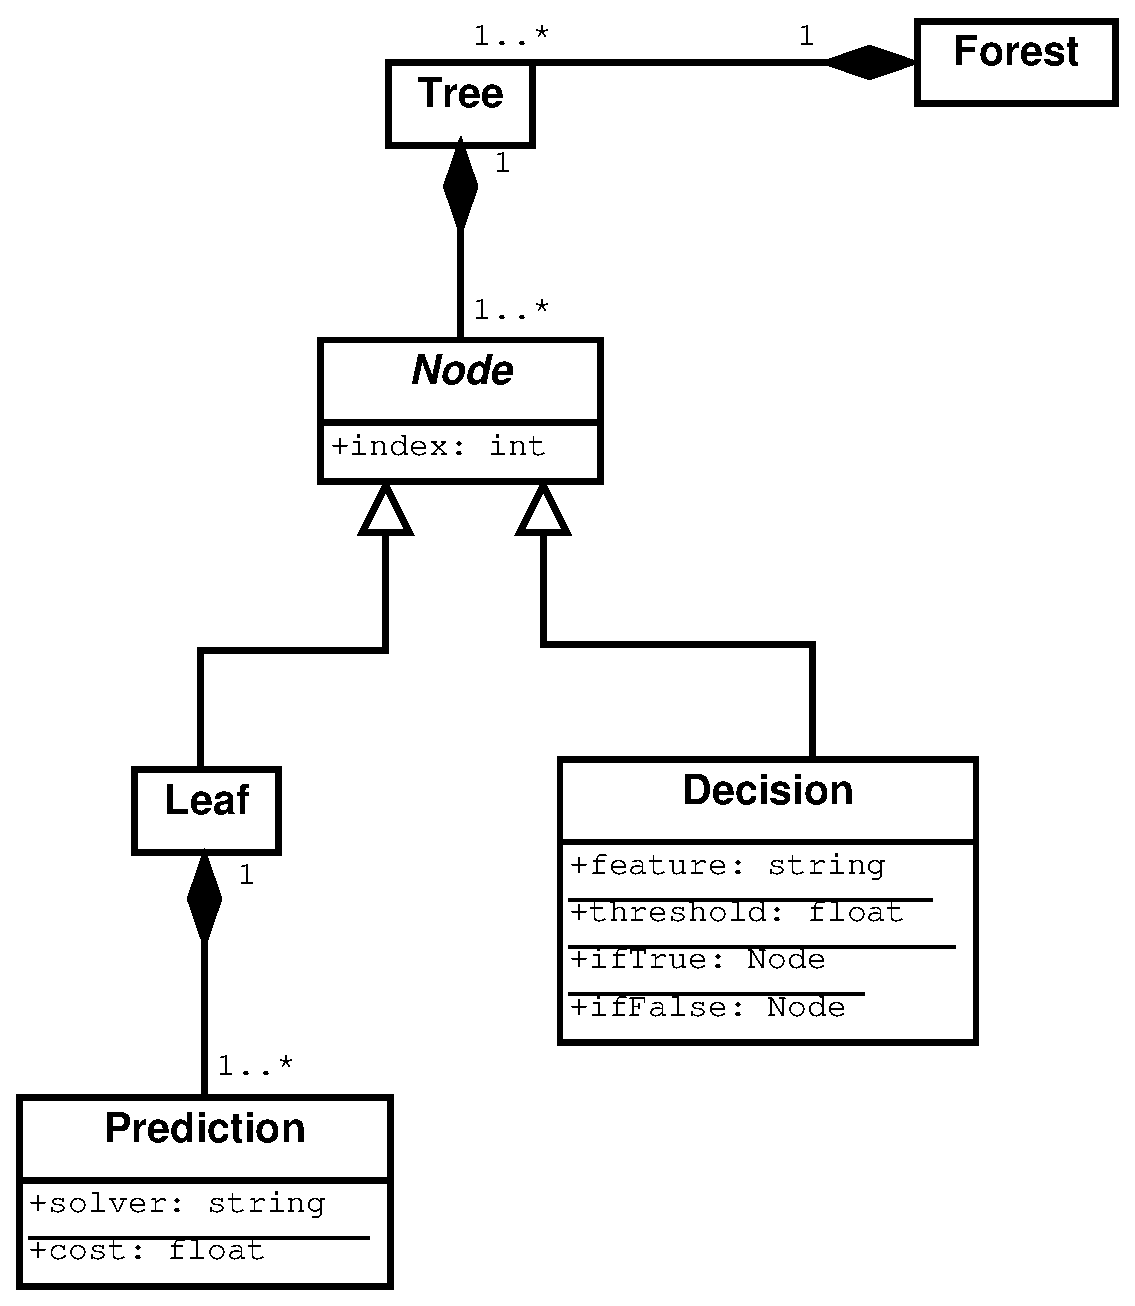
\includegraphics[width=0.8\linewidth]{Figures/data}
\caption[Data design for JSON encoding]{Data design for JSON encoding}
\label{fig:json}
\end{figure}
%
%
%\begin{tabularx}{0.8\textwidth}{@{}ZcY@{}}
%	$forest$ &:=&  $tree^+$ \\
%	$tree$ &:=& $node^+$ \\
%	$node$ &:=& $leaf\,|\, decision$ \\
%	$leaf$ &:=& $(index, prediction^+)$ \\
%	$decision$ &:=& $(index, feature, threshold, true, false)$ \\
%	$prediction$ &:=& $(solver, cost)$ \\
%	$index$ &:=& \texttt{integer} \\
%	$feature$ &:=& \texttt{string} \\
%	$threshold$ &:=& \texttt{float} \\
%	$true$ &:=& \texttt{integer} \\
%	$false$ &:=& \texttt{integer} \\
%	$solver$ &:=& \texttt{string} \\
%	$cost$ &:=& \texttt{float} \\	
%\end{tabularx}

This JSON schema is designed to be human-readable so that users can define their own simple trees in order to experiment with the effect a particular \texttt{feature} may have.
The \texttt{index} attribute is a unique identifier used when traversing the tree: if the value for \texttt{feature} is less than or equal to \texttt{threshold}, the current focus moves to the \texttt{Node} with the value of \texttt{ifTrue}, or to \texttt{ifFalse} if it is greater.
This process continues until a \texttt{Leaf} node is encountered and each solver's cost \texttt{Prediction} is returned.

\sloppypar
Fig. \ref{fig:Chapter5} shows \where's design in terms of OCaml modules.
The functions exposed by the interface files (\texttt{*.mli}) are listed in Appendix \ref{App:interfaces}. 
Upon installation of \where, \texttt{forest.json} is read in by \texttt{print\_tree.ml} and an equivalent OCaml array is generated and written to the file \texttt{tree.ml}.
When \texttt{make\_predictions.ml} is provided with a vector of program features by \texttt{where4.ml}, the forest is traversed  in the manner outlined above.
Making the forest available as an OCaml data structure (through the \texttt{tree.mli} interface file) is more efficient than reading in the JSON file at each execution of \where.
Of course, if \texttt{forest.json} changes, \where~needs to be re-installed for these changes to have effect (more information about installing \where~is given in Appendix \ref{App:install}).  


\begin{figure}
	\centering
	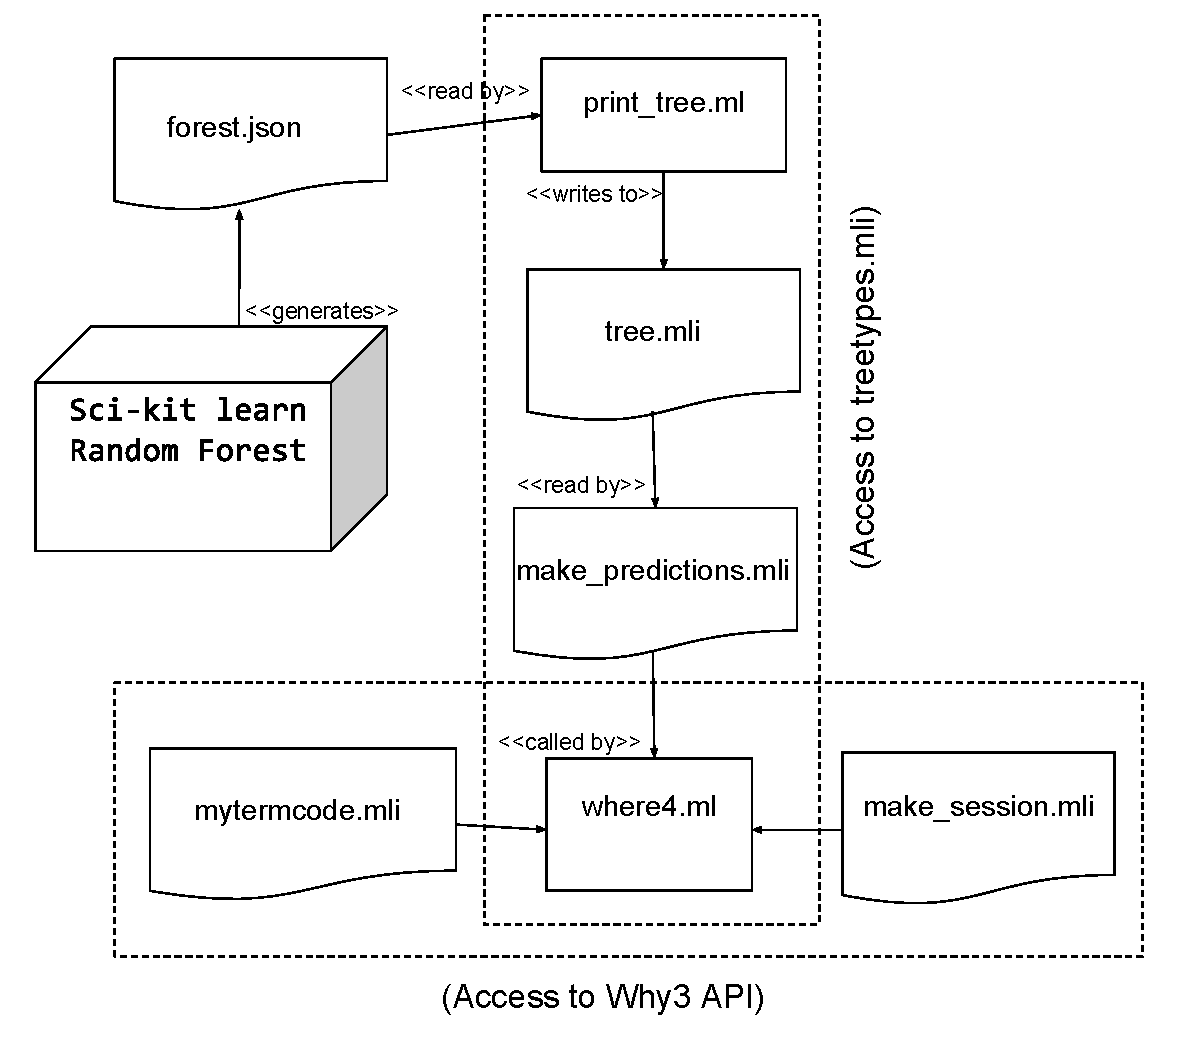
\includegraphics[width=1.0\linewidth]{Figures/Chapter5_stereo}
	\caption[\where~modules]{The organisation of components in \where's design}
	\label{fig:Chapter5}
\end{figure}

\section{Extracting features}

The previous section described \where's use of a tree data structure to predict solver performance given a vector of program features.
A tree is also used to derive these feature vectors from \why~programs: the \why~API is used to traverse the abstract syntax tree (AST) for each PO.
As previously discussed in Sec. \ref{sec:independant}, we use a process similar to that used internally by \why~to extract ``goal shapes'' \cite{why:preserving}.
The \why~OCaml module used to perform this task is named \texttt{termcode.ml} and \where's \texttt{mytermcode.ml} is based upon the same process.

A hash table is maintained while recursively traversing the AST: at each node visited the count of the corresponding feature is incremented in the hash table. 
Any other relevant information (such as function arity, for example) is also recorded before the rest of the tree is traversed. 

\section{Integration with \why}
\label{sec:why3-integration}

\sloppypar
The \texttt{mytermcode.mli}, \texttt{where4.ml} and \texttt{make\_session.mli} files are shown in Fig. \ref{fig:Chapter5} as having access to the \why~API. 
We have already described how \texttt{mytermcode.ml} uses the AST to extract the feature vector.
Other important information required by \why~is gathered by the \texttt{make\_session.ml} module.
For example, this module reads the \why~configuration file to determine which supported SMT solvers are installed locally.
\texttt{make\_session.ml} loads drivers for these solvers and creates a proof session in the current directory. This module reads and type-checks the input file; returning its abstract representation.
These actions are performed using a method described in the \why~manual\footnote{Specifically \url{http://why3.lri.fr/doc-0.87.2/manual005.html\#sec28} (last accessed 16/10/16)} \cite{why:manual}.

\texttt{where4.ml} parses command line options (see Appendix \ref{App:command}) and prints results to the console.
The process it uses to schedule solvers is summarised by Algorithm \ref{algo:where4}.
\where~is available as a stand-alone command-line tool which accepts files written using the WhyML front-end or the Why IVL.
Such a tool is useful as an initial solving step for large batches of files, but it cannot take full advantage of the \why~system.
By following the ``zero click, zero maintenance, zero overhead'' philosophy, we wanted \where's functionality to integrate fully with the \why~user's normal workflow.
To take advantage of the full range of transformations and parsers associated with the \why~system, we decided to make the tool available to be accessed as an individual backend solver.
   
The imitation of an orthodox SMT solver requires a number of modifications and extra files as follows:
\begin{itemize}
	\item An entry to the \texttt{provers-detection-data.conf} configuration file must be made for \why~to recognise \where~ as a supported SMT solver.
	\where's entry lists the command needed to invoke the binary, specifies which version of the tool is supported, and where to find the corresponding driver file.
	\item The driver file must contain regular expressions to parse \where's output, making it comprehensible to \why~(defining the characteristics of a \textit{Valid} output, for example). 
	The driver must also list the printer used by \why~for intermediate files, as well as any transformations which need to be performed to conform to the solver's input language. \where~uses the standard \why~printer and its list of transformations.
	\item The \why~API requires that supplied paths to input files are relative to the current directory. When called via the driver, however, a temporary file is written by the printer and an absolute path is specified. \where~needs to convert this to a relative path in order to read the input file.     
\end{itemize}

These modifications allow \where~to be recognised as an orthodox solver which can be used by \why~through the IDE, on the command-line, or through the OCaml API -- similar to any other supported ATP or SMT tool. 

\section{Summary}

This chapter has presented an overview of the method we used to implement the \where~tool using the \why~OCaml API.
In total, the six statically-written OCaml modules (i.e. not including \texttt{tree.ml}) contain 712 lines of code.
We used OCaml version 4.02.3 for their compilation locally.
The only library we used (in addition to version 0.87.1 of the \why~API) is Yojson\footnote{version 1.2.1 \url{http://mjambon.com/yojson.html}}  to help with parsing the \texttt{forest.json} file. 
The data disk included with this thesis contains all of the source code for \where. 
The files \texttt{install.sh} and \texttt{readme.md} contain useful information about the compilation of these modules and how to satisfy their few dependencies.
The same source files are available online at \url{https://github.com/ahealy19/where4}.

